% !TEX program = xelatex

\documentclass{article}
\usepackage[UTF8]{ctex}
\usepackage[tc]{titlepic}
\usepackage{titlesec}
\usepackage{cite}
\usepackage{fancyhdr}
\usepackage{booktabs}
\usepackage{graphicx}
\usepackage{geometry}
\usepackage[section]{placeins}
\geometry{a4paper,scale=0.8}
\pagestyle{fancy}

\lhead{第 1 次作业\\\today}
\chead{中国科学技术大学\\数学建模课程}

\rhead{Assignment 1\\ {\CTEXoptions[today=old]\today}}
\newcommand{\upcite}[1]{\textsuperscript{\cite{#1}}}

\titleformat*{\section}{\bfseries\Large}
\titleformat*{\subsection}{\bfseries\large}

\title{\bfseries 图像接缝裁剪（Seam Carving）实验报告}
\author{姓名：胡广理 \quad  ID：162 \quad  学号：PB24010500}

\begin{document}
\maketitle
\begin{abstract}
    本报告基于 2007 年的经典论文《Seam Carving for Content-Aware Image Resizing》，实现了一种内容感知的图像缩放算法（接缝裁剪）。不同于传统的线性缩放或直接裁剪，接缝裁剪算法通过计算图像的能量图，利用动态规划算法寻找并移除（或复制）图像中能量最低的连续像素路径（接缝），从而在改变图像长宽比的同时，最大程度地保留了图像中的重要视觉特征和主体内容。
\end{abstract}
\clearpage
% \setcounter{secnumdepth}{1}
 \setcounter{section}{1}
\section*{\centerline{一、前言（问题的提出）}}
\subsection{传统图像缩放的局限性}
    在网页设计和设备适配中，经常需要改变图像的长宽比。最简单直观的方法有“线性伸缩（Scaling）”和“直接裁剪（Cropping）”。然而，线性伸缩会导致图像整体（包括核心主体）发生严重的比例畸变；而直接裁剪虽然不改变主体比例，却会丢失裁剪区域外的图像信息（如关键背景或边缘主体）。

\subsection{内容感知缩放的引入}
    为了克服上述缺陷，我们需要一种既能改变图像长宽比，又能尽可能多地保留图像主要信息且避免主体畸变的方法，“接缝裁剪（Seam Carving）”由此产生。

 \setcounter{section}{2}
\section*{\centerline{二、相关工作}}
    本实验实现参考自 Shai Avidan 和 Ariel Shamir 的论文 \textit{Seam Carving for Content-Aware Image Resizing} (ACM Transactions on Graphics, 2007)。

 \setcounter{section}{3}
\section*{\centerline{三、问题分析}}
    \subsection{能量评估}
    要实现“内容感知”，算法需要区分图像中哪些部分是“重要”的，哪些是“不重要”的。通常，平坦的背景区域视觉信息较少，而包含边缘、纹理特征的区域视觉信息丰富。因此，可以引入“能量函数”来衡量每个像素的视觉重要性。
    \subsection{接缝寻找与移除}
    如果只是简单地移除能量最低的单列或单行像素，会导致图像出现明显的断层。因此需要寻找一条从图像一侧到另一侧的、连贯且总能量最低的像素路径（即接缝 Seam）。

 \setcounter{section}{4}
\section*{\centerline{四、建模的假设}}
    \subsection{局部特征代表视觉重要性}
    假设图像的视觉重要性可以由局部的梯度或拉普拉斯算子响应来准确反映。
    \subsection{单调连贯性}
    假设接缝是 8-连通 的，并且在延伸方向上对每行（或每列）只且只包含一个像素。

 \setcounter{section}{5}
 \section*{\centerline{五、符号说明}}
 \begin{table}[h]
    \caption{\textbf{符号说明}}
    \centering
    \begin{tabular}{ccc}
    \toprule
    符号 & 说明 & 单位 \\
    \midrule
    $I$ & 输入的二维 RGB 图像 & - \\
    $e(x, y)$ & 像素 $(x,y)$ 处的能量值 & - \\
    $s$ & 贯穿图像的一条接缝 (Seam) & - \\
    $M(i, j)$ & 到达位置 $(i,j)$ 时的最小累计能量 & - \\
    \bottomrule
    \end{tabular}
\end{table}

 \setcounter{section}{6}
\section*{\centerline{六、数学模型建立}}
    \subsection{能量图计算}
    能量函数选择基于图像二阶导数的 Laplacian 算子，计算每个通道的响应和的平方作为能量：
    $$e(x, y) = \sum_{c \in \{R,G,B\}} \left( \nabla^2 I_c(x, y) \right)^2$$
    在实验中利用给定的滤波核对图像进行卷积操作实现计算。

    \subsection{动态规划寻找最优接缝}
    以纵向缩放（从上到下）为例，定义累积能量矩阵 $M$，第一行为 $M(1, j) = e(1, j)$，其余行的递推公式为：
    $$M(i, j) = e(i, j) + \min( M(i-1, j-1), M(i-1, j), M(i-1, j+1) )$$
    计算完毕后，矩阵最后一行的最小值即为最优接缝的终点，然后通过回溯（Backtracking）找出整条接缝并将其像素移除。循环执行此操作即可连续缩减图像。

 \setcounter{section}{7}
\section*{\centerline{七、结果（与对比）}}
    \subsection{结果展示}
    使用提供的 Python 框架执行裁剪。如将图片大小缩减，算法能够智能地绕开主要内容的强纹理区（如人物或建筑），而在平滑的背景区域寻找接缝。
    \begin{figure}[htbp]
        \centering
        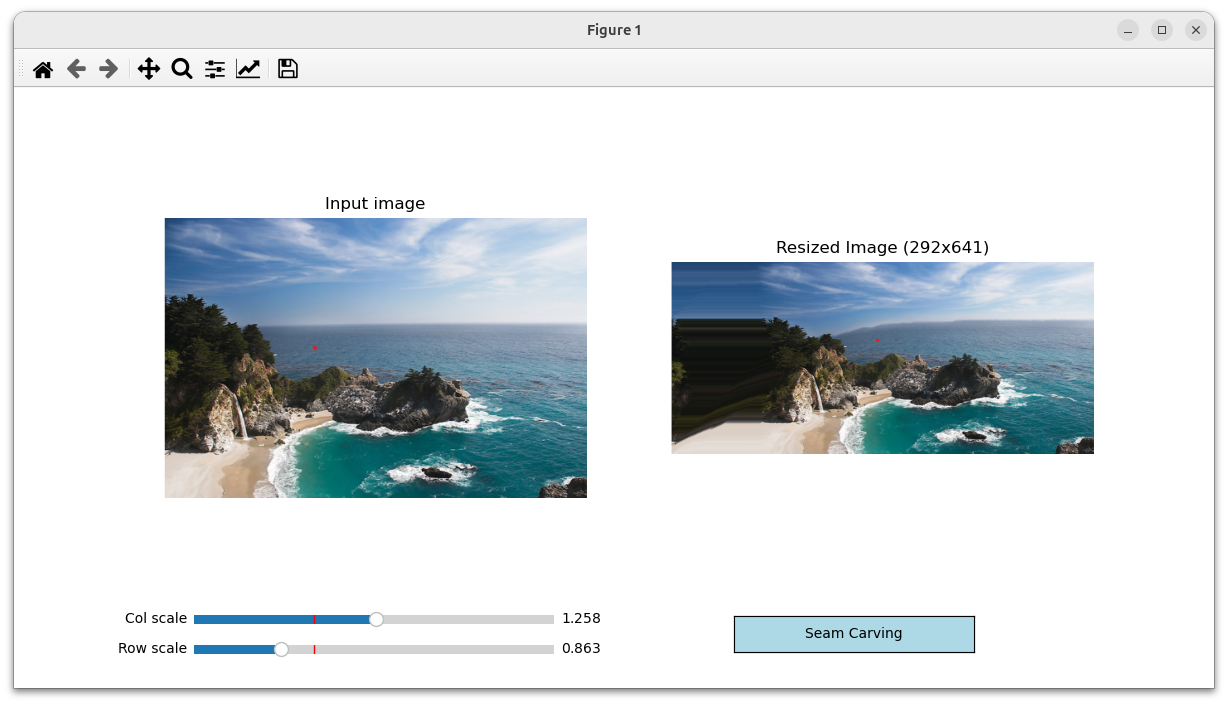
\includegraphics[width=0.8\textwidth]{output_figs/效果展示.png}
        \caption{Seam Carving 缩放结果示例1}
    \end{figure}

    \begin{figure}[htbp]
        \centering
        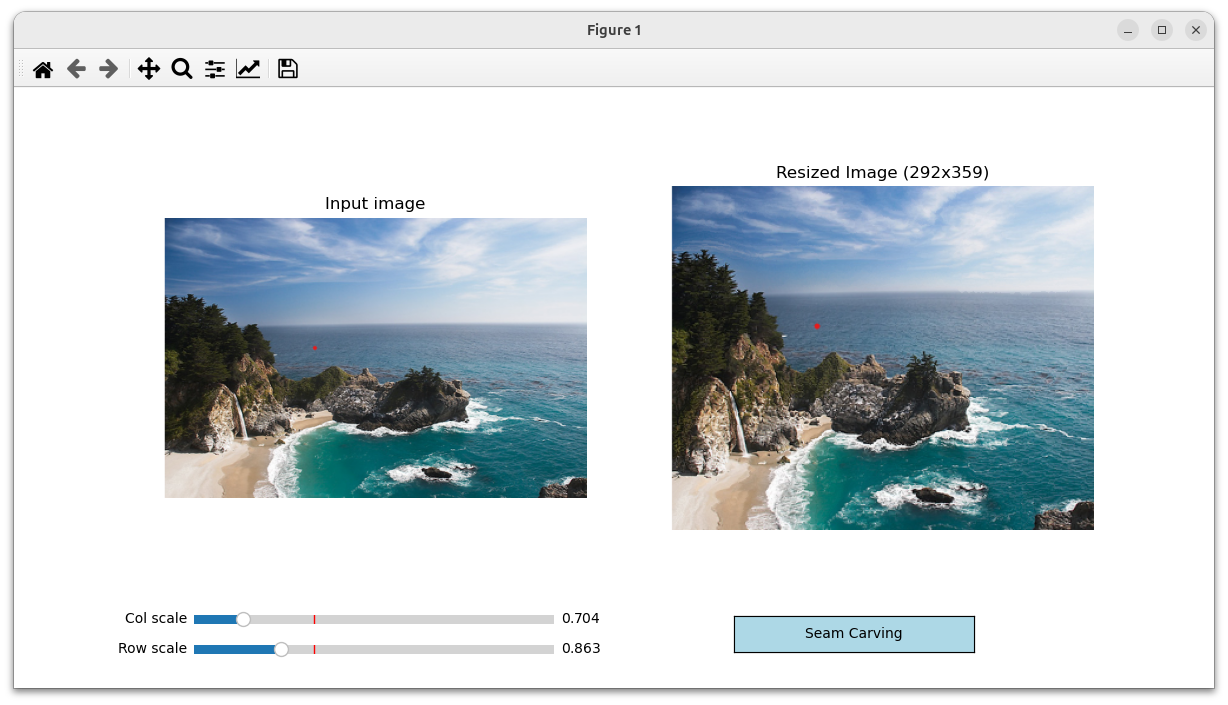
\includegraphics[width=0.8\textwidth]{output_figs/效果展示_2.png}
        \caption{Seam Carving 缩放结果示例2}
    \end{figure}
    
    \subsection{结果对比}
    对比传统的直接截断（直接舍弃一侧的所有像素，丢失大量环境信息）和线性缩放（强制压缩导致高频内容的严重形变），Seam Carving 明显地保留了原始图像的两侧边缘信息和主题比例，在视觉上更为自然和谐。

 \setcounter{section}{8}
\section*{\centerline{八、结论}}
    实验成功实现了 Seam Carving 算法。实验表明，通过能量函数加动态规划的方式来智能选择和去除图像中的无价值连续像素（接缝），能够在绝大数情形下实现优于传统缩放方法的内容感知裁剪效果。  

 \setcounter{section}{9}
\section*{\centerline{九、问题}}
    1. 计算效率：使用 Python 实现的多重循环容易产生性能瓶颈。我在实现中对邻域能量搜索进行了向量化操作（利用 `numpy.pad` 和 `numpy.argmin`），显著提升了查找速度。
    2. 算法局限：如果图片背景与前景都充满大量且密集的纹理特征，Seam Carving 也会被迫破坏重要特征并产生可见的伪影（artifacts）。  

\bibliographystyle{ieeetr}
\bibliography{refer}

\end{document}